\section{Cursograma Producci\'on}
\begin{center}
 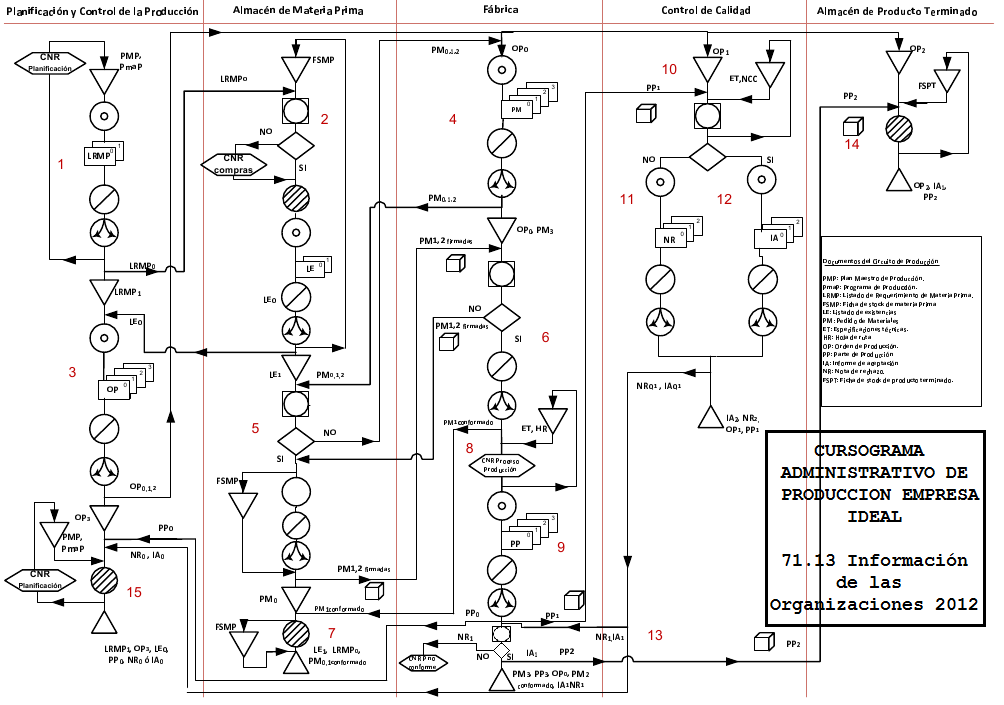
\includegraphics[angle=90,scale=0.95,keepaspectratio=true]{./Circuitos-Teoricos/Produccion/Images/cursograma-produccion.png}
 % cursograma-produccion.png: 1004x705 pixel, 96dpi, 26.56x18.65 cm, bb=0 0 753 529
\end{center}

\section{Procedimiento de Producci\'on}
\begin{center}
 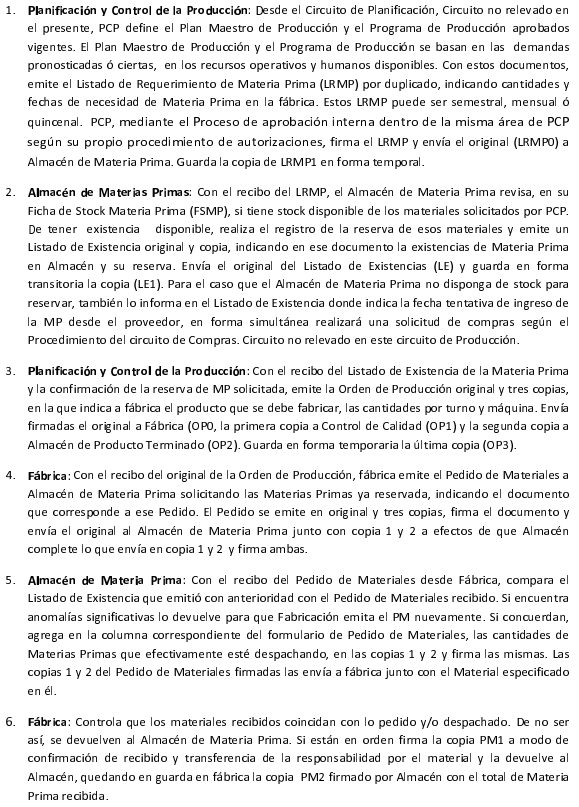
\includegraphics[keepaspectratio=true]{./Circuitos-Teoricos/Produccion/Images/procedimiento-produccion.png}
 % procedimiento-produccion.png: 579x807 pixel, 96dpi, 15.32x21.35 cm, bb=0 0 434 605
\end{center}
\begin{center}
 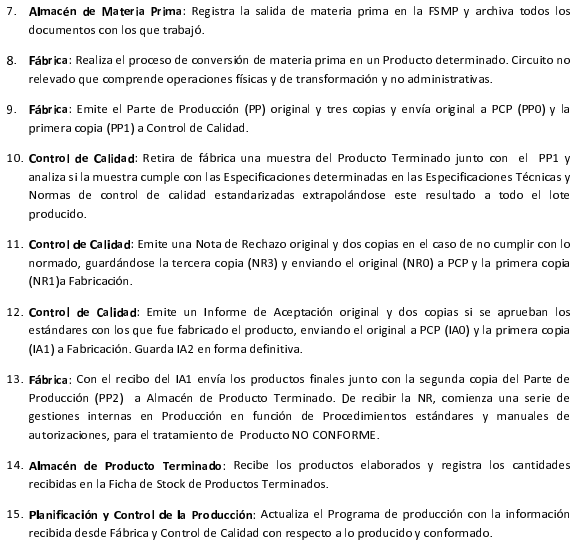
\includegraphics{./Circuitos-Teoricos/Produccion/Images/procedimiento-produccion-2.png}
 % procedimiento-produccion-2.png: 576x545 pixel, 96dpi, 15.24x14.42 cm, bb=0 0 432 409
\end{center}

\pagebreak
\section{Cursograma de Producci\'on (con numeración para el manual)}
\subsection{Manual del Cursograma de Producci\'on}

\begin{center}\textbf{Sectores intervinientes}\end{center}
\begin{itemize}
  \item Planificaci\'on y Control de Producci\'on.
  \item Almac\'en de Materia Prima.
  \item F\'abrica.
  \item Control de Calidad.
  \item Almac\'en de Producto Terminado.
\end{itemize}

\begin{center}
  \textbf{Documentos}
  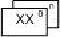
\includegraphics{./Images/Simbolos/simbolo-Documentos.png}
\end{center}
\begin{enumerate}
  \item Listado de Requerimientos de Materia Prima (LRMP).
  \item Orden de Producci\'on (OP).
  \item Listado de Existencia (LE).
  \item Pedido de Materiales (PM).
  \item Parte de Producci\'on (PP).
  \item Nota de Rechazo (NR).
  \item Informe de Aceptaci\'on (IA).
\end{enumerate}

\begin{center}
  \textbf{Emisión de Documentos}
  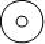
\includegraphics{./Images/Simbolos/simbolo-Emision-de-Documentos.png}
\end{center}
\begin{enumerate}
  \item Planificaci\'on y Control de la Producci\'on: emite el LRMP, original y copia.
  \item Planificaci\'on y Control de la Producci\'on: emite la OP, original y tres copias. 
  \item Almac\'en de Materia Prima: emite un LE, original y copia.
  \item F\'abrica: emite el PM, original y tres copias.
  \item F\'abrica: emite el PP, original y tres copias.
  \item Control de Calidad: emite una NR, original y dos copias.
  \item Control de Calidad: emite un IA, original y dos copias.
\end{enumerate}

\begin{center}
  \textbf{Firma}
  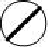
\includegraphics{./Images/Simbolos/simbolo-Firma.png}
\end{center}
\begin{enumerate}
  \item Planificaci\'on y Control de la Producci\'on: firma LRMP original.
  \item Planificaci\'on y Control de la Producci\'on: firma OP original y las dos primeras copias.
  \item Almac\'en de Materia Prima: firma LE original.
  \item Almac\'en de Materia Prima: firma PM primera y segunda copia.
  \item F\'abrica: firma PM original, primera y segunda copia.
  \item F\'abrica: firma PM primera copia conformada.
  \item F\'abrica: firma PP original y las dos primeras copias.
  \item Control de Calidad: firma NR original y copia.
  \item Control de Calidad: firma IA original y copia.
\end{enumerate}

\begin{center}
  \textbf{Distribución}
  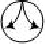
\includegraphics{./Images/Simbolos/simbolo-Distribucion.png}
\end{center}
\begin{enumerate}
  \item Planificaci\'on y Control de la Producci\'on: distribuye LRMP original a Almac\'en de Materia Prima; y converva la copia.
  \item Planificaci\'on y Control de la Producci\'on: distribuye OP original a F\'abrica, la primera copia a Control de Calidad y la segunda copia a Almac\'en de Producto Terminado; conserva la \'ultima copia.
  \item Almac\'en de Materia Prima: distribuye LE original a Planificaci\'on y Control de la Producci\'on; conserva la copia.
  \item Almac\'en de Materia Prima: distribuye PM primera y segunda copia a F\'abrica; conserva el original. \item F\'abrica: distribuye PM original y las dos primeras copias a Almac\'en de Materias Primas; conserva la \'ultima copia.
  \item F\'abrica: distribuye PM primera copia a Almac\'en de Materias Primas. 	
  \item F\'abrica: distribuye PP original a Planificaci\'on y Control de la Producci\'on, la primera copia a Control de Calidad, y la segunda copia a Almac\'en de Producto Terminado; conserva la \'ultima copia.
  \item Control de Calidad: distribuye NR original a Planificaci\'on y Control de la Producci\'on y la primera copia a F\'abrica; conserva la segunda copia.
  \item Control de Calidad: distribuye IA original a Planificaci\'on y Control de la Producci\'on y la primera copia a F\'abrica; conserva la segunda copia.
\end{enumerate}

\begin{center}
  \textbf{Almacenamiento Transitorio}
  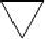
\includegraphics{./Images/Simbolos/simbolo-Almacenamiento-Transitorio.png}
\end{center}
\begin{enumerate}
  \item Planificaci\'on y Control de la Producci\'on: almacena de manera transitoria Plan Maestro de Producci\'on (PMP) y Programa de Producci\'on (PmaP).
  \item Planificaci\'on y Control de la Producci\'on: almacena de manera transitoria LRMP copia.
  \item Planificaci\'on y Control de la Producci\'on: almacena de manera transitoria OP tercera copia.
  \item Planificaci\'on y Control de la Producci\'on: almacena de manera transitoria PMP y PmaP.
  \item Almac\'en de Materia Prima: almacena de manera transitoria Ficha de Stock de Materia Prima (FSMP).
  \item Almac\'en de Materia Prima: almacena de manera transitoria LE copia.
  \item Almac\'en de Materia Prima: almacena de manera transitoria FSMP.
  \item Almac\'en de Materia Prima: almacena de manera transitoria PM original.  
  \item Almac\'en de Materia Prima: almacena de manera transitoria FSMP.
  \item F\'abrica: almacena de manera transitoria OP original y PM tercera copia.
  \item F\'abrica: almacena de manera transitoria Especificaciones t\'ecnicas (ET) y Hoja de Ruta (HR).
  \item Control de Calidad: almacena de manera transitoria OP primera copia.
  \item Control de Calidad: almacena de manera transitoria ET y Normas de Control de Calidad (NCC).
  \item Almac\'en de Producto Terminado: almacena de manera transitoria OP segunda copia.
  \item Almac\'en de Producto Terminado: almacena de manera transitoria Ficha de Stock de Producto Terminado (FSPT).
\end{enumerate}

\begin{center}
  \textbf{Control y verificación}
  
\includegraphics{./Images/Simbolos/simbolo-Control-y-Verificacion.png}
\end{center}
\begin{enumerate}
  \item Almac\'en de Materia Prima: controla y verifica si tiene stock disponible de los materiales solicitados por Planificaci\'on y Control de la Producci\'on, comparando LRMP recibido y FSMP.
  \item Almac\'en de Materia Prima: controla y verifica si concuerda el pedido de materiales, comparando PM recibido de F\'abrica y el LE emitido anteriormente.
  \item F\'abrica: controla y verifica si los materiales recibidos coincidan con lo pedido y/o despachado.
  \item Control de Calidad: controla y verifica si la muestra del Producto Terminado recibida cumple con las especificaciones determinadas en las ET,
\end{enumerate}

\begin{center}
  \textbf{Decisión}
  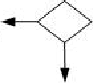
\includegraphics{./Images/Simbolos/simbolo-Decision.png}
\end{center}
\begin{enumerate}
  \item Almac\'en de Materia Prima: 
  \item Almac\'en de Materia Prima: 
  \item F\'abrica: 
  \item F\'abrica: 
  \item Control de Calidad: 
\end{enumerate}

\begin{center}
  \textbf{Operación}
  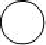
\includegraphics{./Images/Simbolos/simbolo-Operacion.png}
\end{center}
\begin{enumerate}
  \item Almac\'en de Materia Prima:
\end{enumerate}

\begin{center}
  \textbf{Registro}
  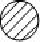
\includegraphics{./Images/Simbolos/simbolo-Registro.png}
\end{center}
\begin{enumerate}
  \item Planificaci\'on y Control de la Producci\'on: registra
  \item Almac\'en de Materia Prima: registra la reserva de materias primas en el LE.
  \item Almac\'en de Materia Prima: registra la salida de materia prima en la FSMP.
  \item Almac\'en de Producto Terminado: registra las cantidades recibidas de productos elaborados en la FSPT.
\end{enumerate}

\begin{center}
  \textbf{Almacenamiento definitivo}
  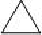
\includegraphics{./Images/Simbolos/simbolo-Almacenamiento-Definitivo.png}
\end{center}
\begin{enumerate}
  \item Planificaci\'on y Control de la Producci\'on: almacena de manera definitiva LRMP copia, OP tercera copia, LE original, PP original y NR original o IA original seg\'un corresponda.
  \item Almac\'en de Materia Prima: almacena de manera definitiva LE copia, LRMP original, PM original y primera copia conformada. 
  \item F\'abrica: almacena de manera definitiva PM tercera copia, PP tercera copia, OP original, PM segunda copia conformada y NR copia o IA copia seg\'un corresponda.
  \item Control de Calidad: almacena de manera definitiva OP primera copia, PP primera copia y IA segunda copia o NR segunda copia seg\'un corresponda.
  \item Almac\'en de Producto Terminado: almacena de manera definitiva OP segunda copia, IA primera copia y PP segunda copia.
\end{enumerate}

\begin{center}
  \textbf{Circuito no relevado}
  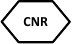
\includegraphics{./Images/Simbolos/simbolo-CNR.png}
  % simbolo-CNR.png: 73x44 pixel, 96dpi, 1.93x1.16 cm, bb=0 0 55 33
\end{center}
\begin{enumerate}
  \item Planificaci\'on y Control de la Producci\'on: Planificaci\'on.
  \item Almac\'en de Materia Prima: Compras.
  \item F\'abrica: Proceso Producci\'on.\
  \item F\'abrica: Tratamiento de Producto NO CONFORME.
\end{enumerate}

\pagebreak
\section{Formularios de Producci\'on}

\subsection{Orden de Producci\'on}
\begin{center}
 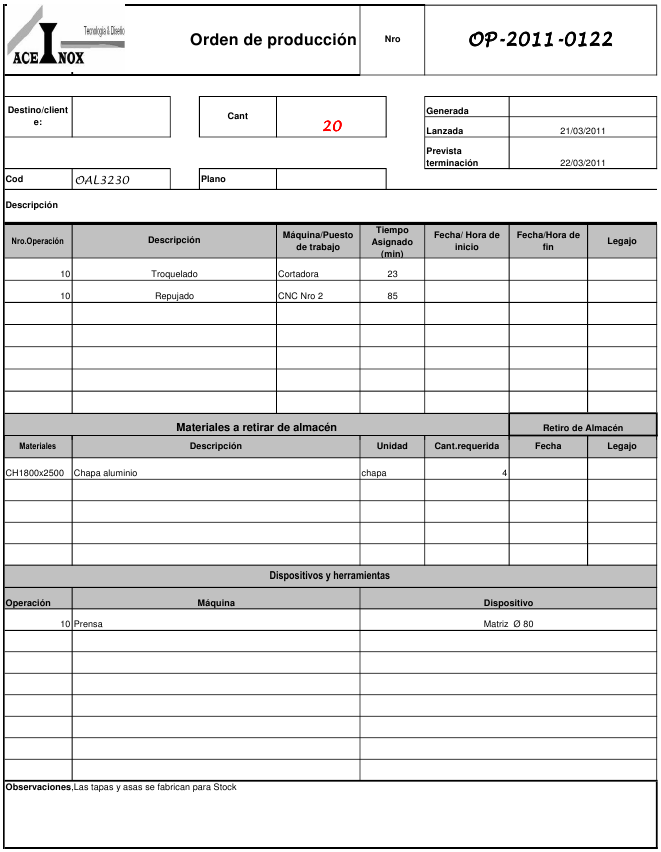
\includegraphics[scale=0.9,keepaspectratio=true]{./Circuitos-Teoricos/Produccion/Images/orden-de-produccion.png}
 % orden-de-produccion.png: 661x852 pixel, 96dpi, 17.49x22.54 cm, bb=0 0 496 639
\end{center}

\subsubsection{Descripción}
\emph{\textbf{TODO}}

\pagebreak
\subsection{Hoja de Ruta}
\begin{center}
 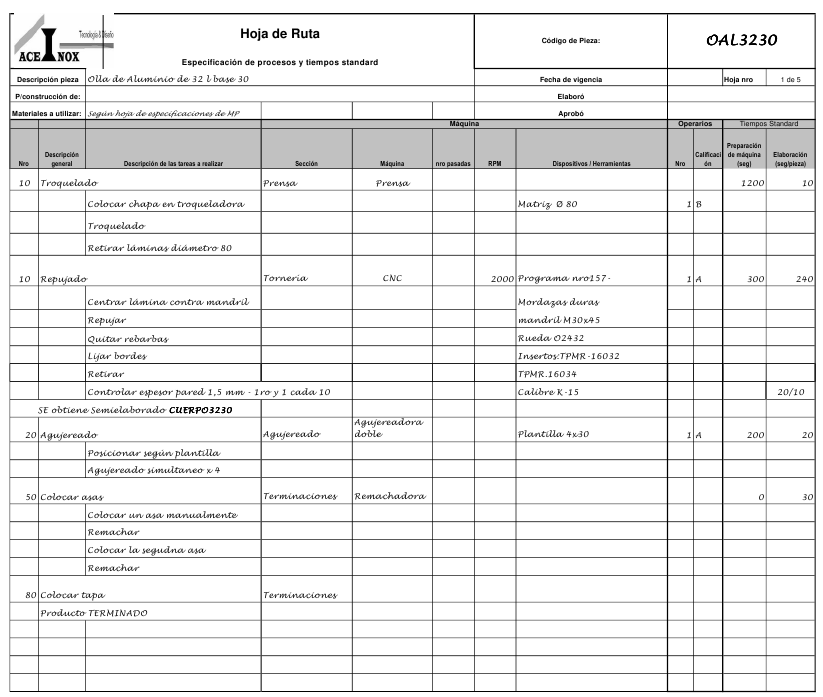
\includegraphics[angle=90,scale=0.95,keepaspectratio=true]{./Circuitos-Teoricos/Produccion/Images/hoja-de-ruta.png}
 % hoja-de-ruta.png: 823x697 pixel, 96dpi, 21.77x18.44 cm, bb=0 0 617 523
\end{center}

\subsubsection{Descripción}
\emph{\textbf{TODO}}

\pagebreak
\section{Normas de control interno generales y específicas de Producci\'on}
\emph{\textbf{TODO}}

\subsection{Normas Específicas}
\emph{\textbf{TODO}}
